\documentclass[11pt, english, fleqn, DIV=15, headinclude]{scrartcl}

\usepackage[bibatend, color]{header}

\hypersetup{
    pdftitle=
}

\ihead{English panels for laundy appliances in FZ Jülich Guest house}
\ohead{Page \thepage}
\ifoot{Made by Martin Ueding (mu@martin-ueding.de) with Inkscape in 2015. If
you want the PDF or SVG file, just email me. This document is completely
independent of the FZ Jülich and the guest house management.}
\cfoot{}

%\subject{}
\title{}
%\subtitle{}
\author{
    Martin Ueding \\ \small{\href{mailto:mu@martin-ueding.de}{mu@martin-ueding.de}}
}

\begin{document}

\section*{Washing machines}

If you have no idea what to do, “easy-care” with \SI{40}{\celsius} should be
fine for most clothes.

\subsection*{Siemens}
\includegraphics[width=\linewidth]{Washing-Siemens-1.pdf}

\subsection*{AEG}
\includegraphics[width=\linewidth]{Washing-AEG-1.pdf}

\subsection*{Zanussi}
\includegraphics[width=\linewidth]{Washing-Zanussi-1.pdf}

\subsection*{Miele}
\includegraphics[width=\linewidth]{Washing-Miele-1.pdf}

\section*{Drying machines}

\subsection*{Miele 1}

\includegraphics[width=\linewidth]{Dryer-Miele-1.pdf}

\subsection*{Miele 2}

\includegraphics[width=\linewidth]{Dryer-Miele-2.pdf}


\end{document}

% vim: spell spelllang=de tw=79
